
%Here is the link to the lecture slides for this deliverable
%https://gitlab.cas.mcmaster.ca/courses/capstone/-/blob/main/Lectures/L02_ProbStateAndGoals/ProbStateGoalsDevPlan.pdf

\documentclass{article}


\usepackage{hyperref} %for referencing tables and links
\hypersetup{
    colorlinks=true,
    linkcolor=blue, %Makes any referencing links blueeeeee
    filecolor=magenta,      
    urlcolor=cyan,
    }
\usepackage{blindtext}
\usepackage{tabularx}
\usepackage[margin=1.25in]{geometry}
\usepackage{indentfirst} %this indents the first line after a section/subsection
\usepackage{graphicx}%to add photos
\usepackage{float} %for formating table spacing

\title{\textbf{4TB6: SRS}\\
\addlinespace
\addlinespace
\addlinespace
\addlinespace
\large \textbf{Stonecap Solutions - Smart Serve}
\addlinespace
\addlinespace
\addlinespace
\addlinespace}

\author{Max Turek $turekm$\\Ryan Were $werer$\\Sam Nusselder $nusselds$\\Peter Minbashian $minbashp$\\David Bednar $bednad1$}

\date{10/05/2022}

\begin{document}

\maketitle
\newpage
\tableofcontents
\listoffigures
\listoftables

\newpage

    % Revision History table
    \begin{table}[hp]
    \caption{Revision History} \label{TblRevisionHistory}
    \hline
        \begin{tabularx}{\textwidth}{llX}
        \toprule
        \textbf{Date} & \textbf{Developer(s)} & \textbf{Change}\\
        \midrule
        & Max Turek & \\
        & Sam Nusselder &  \\
        10/05/22 & Ryan Were & Initial Draft\\
        & Peter Minbasian & \\
        & David Bednar & \\
        \bottomrule
        \hline
        \toprule
        \midrule
        11/02/22 & Sam Nusselder & Added new functional requirements ODR14 - ODR18 from Hazard Analysis Doc\\
        \bottomrule
        \hline
        \toprule
        \midrule
        11/02/22 & Max Turek & Changed glass to cup for definitions, terms, acronyms and abbreviations table \\
        \bottomrule
        \hline
        \toprule
        \midrule
        01/04/23 & Max Turek & Updated document to reflect issues from other teams. Removed ODR7, edited PR7 \&\ PR8, rationale added for QR1 and citation added for HSR3. Added rationale to some requirements, added list of tables and figures and added value range for monitored variables\\
        \bottomrule
        \hline
         03/31/23 & Ryan Were & Revised Functional Requirement numbers so they are sequential. Removed functional requirements that are no longer relevant\\
        \hline
        \end{tabularx}
    \end{table}

\newpage
\section{Introduction}
\subsection{Purpose} % not on rubric, might be good to have tho
    % Problem Explanation
    Stonecap Solutions aims to solve existing issues in the billion dollar bartending industry relating to the process of fulfilling drink orders. Bars are often busy with many orders being processed through a mental queue by bartenders. This can result in long wait times. Furthermore, many restaurants and bars are susceptible to being understaffed, further exasperating this issue. Cocktails and other drinks are imprecisely made, varying in volume and consistency. When bartenders are rushing around to make these drinks, the risk of spilling them arises. If these issues are severe enough, it could result in unsatisfied customers, decreasing business profits. \\

    % Proposed Solution
    Stonecap Solutions aims to solve this problem by developing a drink delivery system that streamlines the process of a customer ordering a drink up to them receiving it. The system would automate the tasks of taking customer orders, making the drinks, and alerting the end user when the drinks are ready. This would result in a system that creates consistent, accurate and timely drinks while avoiding unnecessary spillage.



\subsection{Definitions, Terms, Acronyms and Abbreviations}
    % Table 2
    \begin{center}
    \begin{table}[H]
        \begin{tabular}{ | p{4cm} | p{10cm} | }
        \hline
        \textbf{Term} & \textbf{Definition} \\
        & & 
        \hline
        Drink & Drink will refer to any mixed drink or cocktail made up of many or one ingredient.  \\
        \hline
        Web App & Web application that is used by the customer to order drinks, and used by administrators to monitor the device.\\
        \hline
        Cup & Container that will hold the liquids/ingredients of a drink. \\
        \hline
        Operator & Usually a bartender or manager that is responsible for maintaining the system and has administrative privileges. \\ 
        \hline
        User & Individual that is interacting with the UI and requesting a drink from the system \\
        \hline
        \end{tabular}
    \caption{Table of Definitions, Terms, Acronyms and Abbreviations}
    \label{Table 2}
    \end{table}
    \end{center}


\subsection{Scope}
    The goals of the system are found in Table \ref{Table 3}. These goals have determined the following primary behaviours that make up the scope of the project:

    % Numbered list
    \begin{enumerate}
        \item Ordering Drink: Users are able to interact with a user-interface to order a drink
        \item Creating Drink: Drink is accurately and quickly created
        \item Serving Drink: Customer is notified drink is ready
    \end{enumerate}

    % Table 3
    \begin{center}
    \begin{table}[H]
        \begin{tabular}{ | p{5cm} | p{9cm} | }
        \hline
        \textbf{Goal} & \textbf{Explanation} \\
        & & 
        \hline
        Ease of Communication & End users are able to effectively communicate with Smart Serve. Users understand the status of Smart Serve. This would be measured by all customer orders being fulfilled correctly and all users being informed on their order status.  \\
        \hline
        Ease of Use & System is simple and easy to use for all customers. This would be measured by at least 75 percent of users find the product intuitive to use.\\  
        \hline
        Autonomy & Smart Serve is fully autonomous once starting up. This allows users to interact with Smart Serve without any human interaction. \\  
        \hline
        Consistency & Smart Serve continues to pour a consistent drink after 100 pours. \\  
        \hline
        Accuracy & Smart Serve pours drinks with accurate proportions. This would be measured by checking if the individual ingredients of a drink follow the appropriate proportion (i.e. 1.5 liquid ounces of rum and 4.5 liquid ounces of coke). \\  
        \hline
        Fast Service & Drinks are served to users quickly. One drink is served within 60 seconds. \\  
        \hline
        Operator & The operator had access to the operator controls in the web app. These controls allow the operator to manage ingredients in the web app. \\  
        \hline
        \end{tabular}
    \caption{Project Goals}
    \label{Table 3}
    \end{table}
    \end{center}

    The stretch goals shown in Table \ref{Table 4} were not included in the scope because they are goals that will only be implemented once all the primary project goals are implemented.

    % Table 4
    \begin{center}
    \begin{table}[hp]
        \begin{tabular}{ | p{5cm} | p{9cm} | }
        \hline
        \textbf{Stretch Goal} & \textbf{Explanation} \\ 
        & & 
        \hline
        Self Cleaning & Smart Serve is able to clean all necessary components without human interaction. \\  
        \hline
        Fool Proof & Any risks posed by realistic system malfunctions should be minimized through smart design.\\
        \hline
        Smart Recommendations & Smart Serve can provide drink recommendations. This can be measured by drink recommendations being purchased at least 20 percent of the time.\\
        \hline
        \end{tabular}
    \caption{Stretch Goals}
    \label{Table 4}
    \end{table}
    \end{center}


\subsection{Context Diagram}\\ 

    % Figure 1
    \begin{figure}[H]
    \centerline{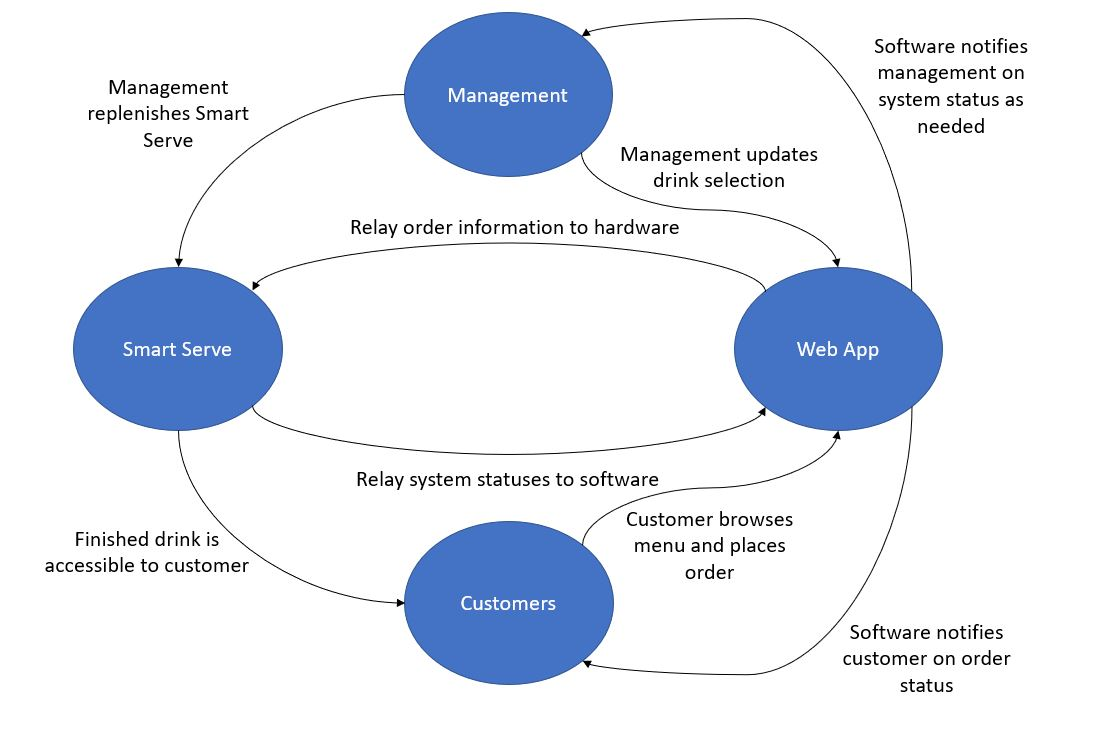
\includegraphics[scale=.75]{ContextDiagram.JPG}}
    \caption{Context Diagram}
    \label{fig}
    \end{figure}

\subsection{Monitored and Controlled Variables}
\subsubsection{Monitored Variables} % variables that go into the hardware
    \begin{itemize}
        \item M\_ingredientReady
        \begin{itemize}
            \item True or False
        \end{itemize}
        \item M\_cupPresent
        \begin{itemize}
            \item True or False
        \end{itemize}
        \item M\_cupEmpty
        \begin{itemize}
            \item True or False
        \end{itemize}
        \item M\_username
        \begin{itemize}
            \item True or False
        \end{itemize}
        \item M\_password
        \begin{itemize}
            \item True or False
        \end{itemize}
        \item M\_alcoholID
        \begin{itemize}
            \item 0-5 range
        \end{itemize}
        \item M\_mixID
        \begin{itemize}
            \item 0-5 range
        \end{itemize}
        \item M\_drinkVolume
        \begin{itemize}
            \item 0-2 range
        \end{itemize}
        \item M\_orderPlaced
        \begin{itemize}
            \item True or False
        \end{itemize}
    \end{itemize}
    
\subsubsection{Controlled Variables} % variables that come out of the hardware
    \begin{itemize}
        \item C\_valveOpen
        \item C\_notification
    \end{itemize}
\subsubsection{System Responses}
    
    \begin{figure}[H]
    \centerline{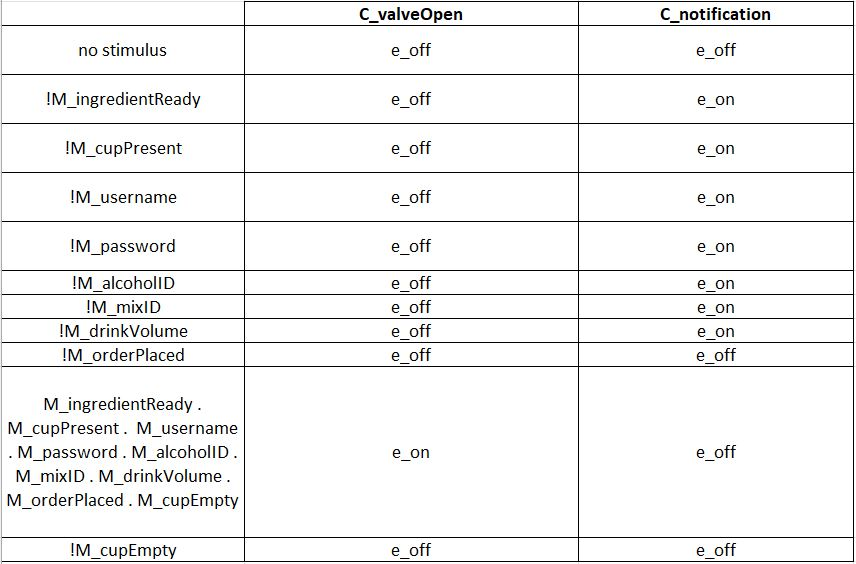
\includegraphics[scale=0.9]{SystemResponse.JPG}}
    \caption{System Response Chart}
    \label{fig}
    \end{figure}

     % Figure 3
    \begin{figure}[H]
    \centerline{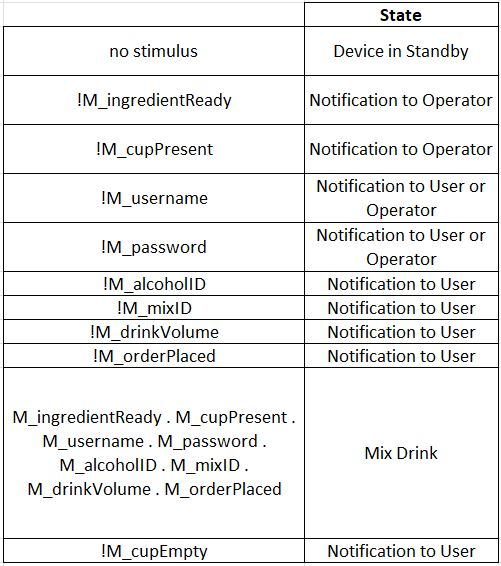
\includegraphics[scale=0.9]{StimulusEffect.JPG}}
    \caption{Stimulus Effect Chart}
    \label{fig}
    \end{figure}

\subsection{Constants}
    \begin{itemize}
        \item Ingredient flow rate
        \item Cup size
        \item Turntable rotation speed
        \item Location of cup
        \item Ingredient vat volume
    \end{itemize}

\subsection{Behaviour Overview}
    Smart Serve is an autonomous system once the user orders a drink. The user can interact with the web app to place an order with Smart Serve. From here the system is entirely autonomous. Once the user is at the front of the queue, the drink will be created and then served where it can be picked up. Smart Serve will remain in standby mode when not in use, and wait for instructions.

\subsection{Stakeholders}
    \begin{itemize}
        \item Stonecap Solutions
        \item Restaurants and business owners that serve drinks
        \item Consumers seeking an autonomous drink creation system
        \item Bartenders
        \item Customers at bars
    \end{itemize}

\section{Project Overview}
\subsection{Normal Operation}
    Smart Serve is intended for users to order drinks and have their drinks robotically made for them. Users will be able to interact with Smart Serve using their phone allowing multiple users to simultaneously order drinks. This will also allow users to socialize with friends while ordering drinks as opposed to waiting in line. Once the order is processed, Smart Serve will begin creating the drink. This process will be completely autonomous. Once the drink is complete, the user will be notified. This will again save the user time waiting in lines for their drink to be made.

\subsection{Undesired Event Handling}
    In the case that an undesired event occurs, Smart Serve should return to a safe state. During the transition into a safe state, Smart Serve should ensure that no harm is caused to the user or itself. This would be done by pausing the current action, notifying the operator to ensure no one is physically interacting with Smart Serve and allowing Smart Serve to return to the home state. The operator would then need to reset Smart Serve and send an alert to Smart Serve to notify that Smart Serve will restart the previous action. This would ensure that the user would still get their drink created at the appropriate spot in queue, while also ensuring the safety of the users and Smart Serve.

\subsection{User Characteristics}
There are two intended users for Smart Serve: Managers and Customers. \\\\
\indent{Managers are grouped as people who intended on using the system to replace bartenders. They own/operate an establishment that sells alcohol. The establishment is busy enough that automating these tasks is warranted to improve service time and reduce labor costs.}\\\\
\indent{Customers would be classified as groups of people who frequently attend establishments that serve alcohol. These customers drink alcohol themselves, most likely drinking cocktails or mixed drinks. They own smartphones and have a basic understanding of modern technology and can navigate through a basic web app.}

\subsection{Constraints}
    Our product can only function within it's given constraints. Some limitations include but not limited to: 
    \begin{itemize}
        \item Reliability of internet service via data or WiFi for UI and Cloud Operations
        \item Liquor laws and regulations involving the service of alcohol
        \item Sanitary regulations pertaining to the service of drinks
    \end{itemize}

\subsection{Assumptions and Dependencies} %not in rubric
    The following assumptions have been made while creating Smart Serve:
    \begin{itemize}
        \item All users are of legal drinking age
        \item All users are in a safe health condition to consume alcohol, including intoxication level
        \item All users have a tab created that is assumed to be paid in full once they have finished ordering all their drinks
        \item Smart Serve will be used in an indoor environment
        \item Ingredient flow rate is kept constant
        \item All cup sizes will be identical
        \item All cups will be plastic
        \item Smart Serve will be kept clean and not restricted due to usage
        \item Smart Serve will always have an internet connection
        \item Smart Serve will always have electrical power
        \item Ingredient viscosity is consistent
    \end{itemize}

\section{Function Requirements}
\subsection{Ordering Drink}
    \noindent\textbf{ODR1.} User can scan QR code launching smart-serve web app \\\\ 
    \textbf{ODR2.} User can access the menu and select drinks to order\\\\
    \textbf{ODR3.} Users can view the placement of their order in the queue \\\\ 
    \textbf{ODR4.} User is notified if drink ingredients are out of inventory\\\\ 
    \textbf{ODR5.} User is notified when their drink is done\\

    \textbf{Rationale:} This is done so the drink does not stay idle while other customers are waiting\\\\
    \textbf{ODR6.} Operator is notified if drink ingredients are out of inventory\\\\
    \textbf{ODR7.} Operator inputs all ingredients available for drinks into the web app\\\\
    \textbf{ODR8.} Operator inputs dispenser location of each ingredient into web app\\
    
    \textbf{Rationale:} This allows for more flexibility with drink mixing and makes the system more universal.\\\\
    \textbf{ODR9.} User gets notified when the drink is ready via web app\\\\
    \textbf{ODR10.} Web app keeps track of drinks made\\

    \textbf{Rationale:} Data is used for analytics to track popular drinks/ingredients or for inventory check\\\\
    \textbf{ODR11.} Server decrypts drink name and gathers ingredients\\\\
    \textbf{ODR12.} User's drink is the same drink they ordered on the app \\\\
    \textbf{ODR13.} User can log in successfully into the app \\\\
    \textbf{ODR14.} User has user permissions  \\\\
    \textbf{ODR15.} Electrical components of high exposure to liquids have waterproof covering\\\\
    \textbf{ODR16.} Have a robust and durable architecture/components\\\\
    \indent\textbf{Rationale:} Bars and pubs can be high-traffic areas resulting in spills and collisions\\

\subsection{Making Drink}
    \noindent\textbf{MDR1.} Hardware receives ingredients from server \\\\
    \textbf{MDR2.} Hardware dispenses the appropriate amount of liquid from respective bottle \\\\
    \textbf{MDR3.} Hardware can detect if a cup is present \\\\
    \textbf{MDR4.} Hardware can detect if the cup is empty or full \\\\
    \textbf{MDR8.} Web app displays that an order is ready so the user can remove it \\\\
    \textbf{MDR9.} Hardware will not start the next order until the completed drink is removed, and a new empty cup is placed in dispensing area \\\\
    \textbf{MDR10.} Hardware does not begin a new drink until the previous drink is removed \\\\

\section{Non-Functional Requirements}
\subsection{Quality requirements of the entire system}
    \noindent\textbf{QR1.} Smart Serve must be robust\\ 
    
    \textbf{Rationale:} During steady state operation, smart serve will satisfy all its functional requirements.\\
\subsection{Look and Feel Requirements}
    \noindent\textbf{LFR1.} The web app must be intuitive and visually appealing \\\\
    \indent\textbf{Rationale:} The least amount of clicks necessary will result in a more user-friendly UI\\\\
    \textbf{LFR2.} Smart Serve must have all electrical and mechanical components concealed \\

\subsection{Usability and Humanity Requirements}
    \subsubsection{Ease of use}
        \noindent\textbf{UHR1.} Smart Serve must serve the drink at a height that is easy to grab for an average adult \\\\
        \textbf{UHR2.} Smart Serve must make grabbing the drink easy for the user, without blockages or inconveniences\\\\
        \textbf{UHR3.} The web app must make it easy to navigate and select drinks\\
    \subsubsection{Ease of learning}
        \noindent\textbf{UHR4.} Finding and gaining access to the web app must be easy \\

\subsection{Performance Requirements}
    \subsubsection{Speed requirement}
        \noindent\textbf{PR1.} The drink must be ready and served within 60 seconds of when the drink began to be made \\\\
        \textbf{PR2.} The web app must be highly responsive to user inputs \\\\
        \textbf{PR3.} The web app must add a users order to the queue of orders within 5 seconds of ordering \\
        \indent\textbf{Rationale:} This requirement is set in order to be comparable to a human creating the same drink\\\
    \subsubsection{Safety critical requirement}
        \noindent\textbf{PR4.} Smart Serve must not release more than 1.1x the amount of expected alcohol \\
        \\ \indent\textbf{Rationale:} Consuming more alcohol than expected can be dangerous for a user \\
    \subsubsection{Precision requirement}
        \noindent\textbf{PR5.} Smart Serve must be able to measure drink ingredients within 10\% of the expected value \\
    \subsubsection{Reliability and availability requirement}
        \noindent\textbf{PR6.} Smart Serve must be able to create the correct drink every time as long as it has the correct ingredients \\
    \subsubsection{Capacity requirement}
        \noindent\textbf{PR7.} Smart Serve must be able to store up to 5 ingredients \\\\
        \textbf{PR8.} Smart Serve must be able to store up to 2 liters of each ingredient \\

\subsection{Operational and Environmental Requirements}
    \subsubsection{Expected physical environment}
        \noindent\textbf{OER1.} Smart Serve must not be exposed to rain or poor weather \\\\
        \textbf{OER2.} Smart Serve must be placed upright on a flat surface \\
    \subsubsection{Expected technological environment}
        \noindent\textbf{OER3.} Smart Serve must have access to wifi \\\\
        \textbf{OER4.} Smart Serve must have access to electricity \\\\
        \textbf{OER5.} The user must have internet access to the same wifi network as Smart Serve and a device to access the web app \\
    \subsubsection{Partner applications}
        \noindent\textbf{OER6.} Smart Serve must be equipped with a cup to serve a drink \\\\

\subsection{Maintainability and Support Requirements}
    \subsubsection{Maintainability}
        \noindent\textbf{MSR1.} Smart Serve should be cleaned once every day \\\\
        \textbf{MSR2.} Smart Serve must be restocked with new ingredients to be able to serve drinks \\
    \subsubsection{Special Maintenance Conditions} 
        \noindent\textbf{MSR3.} No electronic or water-sensitive components of Smart Serve can get wet during cleaning \\\\
        \textbf{MSR4.} The operator must add the ingredients to the web app when Smart Serve is restocked \\
    \subsubsection{Portability}
        \noindent\textbf{MSR5.} Smart Serve must be modular and easy to transport \\\\
        \textbf{MSR6.} Smart Serve must be under 100 pounds \\\\
        \indent\textbf{Rationale:} This is done so it can be carried with one to two people with ease\\

\subsection{Security Requirements}
    \textbf{SR1.} Communication between the web app and Smart Serve must be secure \\\\
    \textbf{SR2.} The operator must be responsible for correctly operating the machine and restocking ingredients \\\\
    \textbf{SR3.} The user must provide identification and be of drinking age to order and receive a drink from Smart Serve \\\\

\subsection{Cultural and Political Requirements}
    \noindent{Not applicable} \\
\subsection{Legal Requirements}
    \noindent\textbf{LR1.} Smart Serve must only be used in countries where alcohol is legal \\\\
    \textbf{LR2.} Smart Serve must not produce a drink that is consumed by persons under the drinking age \\\\
    \textbf{LR3.} The operator of Smart Serve is liable for all drinks served \\

\subsection{Health and Safety Requirements}
    \noindent\textbf{HSR1.} Smart Serve or the operator must not serve a drink to someone who is dangerously intoxicated \\\\
    \textbf{HSR2.} Smart Serve should not be operational near unsupervised persons under the drinking age \\\\
    \textbf{HSR3.} Smart Serve or the operator must not serve more than 2 drinks per hour to one user\textsuperscript{[1]} \\\\
    \textbf{HSR4.} No electrical component can come into contact with any fluid \\

\section{Likely Changes to Requirements}
\subsection{Machine Improvements}
    \noindent Although the first design of the machine has a degree of durability and ease of maintenance, a goal within the group is to have the machine not only be able to last longer but allow for even less maintenance/care. This can be accomplished with the following new requirements. \\\\
    \textbf{RLC 1:} Incorporate self-cleaning after every drink is made\\\\
    \textbf{RLC 2:} Design system hardware to have a high water resistance\\\\
    \textbf{RLC 3:} Have the system be more robust to lessen the risk of impact damage\\\\
    \textbf{RLC 4:} Machine sends specific error codes to the operator to inform why the machine is breaking\\
\subsection{Data Analytics}
    \noindent With the current design, the system will use basic Data Analytics to track information like popular drinks and stock of ingredients. A likely change will be to take advantage of the data to produce the following requirements. \\\\
    \textbf{RLC 5:} Purchasing patterns are used to track optimal inventory \\\\
    \textbf{RLC 6:} Analysis of user data is used to find correlations with drink orders to derive optimal drink mixes or drink recommendations\\

\section{Unlikely Changes to Requirements}
    \noindent\textbf{UCR 1:} No new input of human interaction for base functionality. \\

    \noindent\textbf{Justification: }One of the main purposes of this project is to incorporate more automation into the bartending profession. The requirements outlined reflect that. Any increase in human interference for base functionality will contradict this purpose. \\\\
    \noindent\textbf{UCR 2:} Application will \textbf{always} comply with safety and the law. \\

    \noindent\textbf{Justification: }Due to the device serving, it is important that all government regulations be followed. Misuse of the device could result in lawsuits, jail time, injury, or death. While handling alcohol, it is of the utmost importance that the device follows the substance's regulations.\\\\
    \noindent\textbf{UCR 3:} Web Application must be user-friendly and very simple to use.  \\

    \noindent\textbf{Justification: }Theoretically, the system can be a substitute for the simplistic traditional human-to-human interaction of asking for a drink. The app must be at least as straightforward as the traditional method.\\\\

    \noindent\textbf{UCR 4:} System must be able to create drinks with a high level of preciseness and consistency as an average bartender.  \\

    \noindent\textbf{Justification: }With the system replacing the need for a bartender, it must be able to (at the very least) create drinks with both the appropriate measurements and a strong degree of consistency.\\\\
    \noindent\textbf{UCR 5:} Maintenance of Smart Serve must be simplistic.  \\

    \noindent\textbf{Justification: }It must be assumed that a large demographic of operators of Smart Serve do not have a background in technology. The maintenance of the device should be straightforward, with limited technological experience required. 
\newpage
\section{References}
   1. Alcohol and your body. [Online]. Available: https://shop.ucsc.edu/alcohol-other-drugs/alcohol/your-body.html. [Accessed: 04-Jan-2023]. 
\newpage
\section{Appendixes}
\subsection{Reflection}
    %What knowledge and skills will the team collectively need to acquire to successfully complete this capstone project? Examples of possible knowledge to acquire include domain-specific knowledge from the domain of your application, software engineering knowledge, mechatronics knowledge or computer science knowledge. Skills may be related to technology, writing, presentation, team management, etc. You should look to identify at least one item for each team member.

    %For each of the knowledge areas and skills identified in the previous question, what are at least two approaches to acquiring the knowledge or mastering the skill? From the identified approaches, which will each team member pursue, and why did they make this choice?

    \noindent\textbf{Max Turek:} \\
    \indent{As a mechatronics engineer, we get experienced with software, electrical and mechanical aspects but never become experts in one. Therefore, one skill I will need to learn how to acquire is working on mechanical and electrical systems specifically pumps for transporting fluids. Furthermore, I will need to understand front-end and web development more in order to launch and troubleshoot our web app that supports the user interface.}\\
    \indent{One way I find is best for acquiring new knowledge is youtube videos. It is possible to find a video explaining almost any skill now a days. The other channel of acquiring knowledge would to speak to alumni and friends that have completed a mechatronics capstone. I have many friends that are knowledgeable in software and hardware that are able to provide consultation and advice.} \\
    \newline
    \textbf{Sam Nusselder:} \\
    \indent{The team will need to have a strong understanding of mechanical, electrical and software components as well as the capabilities of integrating these systems. Mechanical and electrical systems related to delivering and controlling fluid flow will be required. Software knowledge with web-based applications will also be needed to develop an interface so users are able to interact with Smart Serve. Team management and group work skills will be needed in order to ensure a successful working team of 5 members. It will be important to make sure everyone always has a task to work on while also ensuring everyone understands the "bigger" picture and is aware of the long-term goals.}\\
    \indent{Some approaches to acquiring a strong understanding of mechanical, electrical and software components is to review any applicable course work and to do more research online to learn about these topics. All team members will need knowledge in all of these areas, so they will need to pursue which ever approach works best for them as they feel they need a stronger understanding. To acquire better team work skills, team members can look past on their individual previous group work experiences and learn from things that went well and things that didn't. Another approach to improve team work skills is to speak with other current groups to learn and understand how they work effectively as a team. All team members can pursue the approach that works best for them. Not everyone has great team work experience to learn from, so this is where the second approach would be more effective.}\\\\
     \textbf{Peter Minbashian:} \\
     \indent{As a computer engineering student at McMaster, a majority of my foundational knowledge, surrounding technology, revolves around embedded software. Although that is applicable to this project, I present not much value to the web development portion. Therefore, it would be best that for me to learn more about web development. Not only will this entail learning the basics (JavaScript, HTML, CSS) but also learning specific tools required for this project. This includes how to incorporate user log-in functionality on a website, connecting a website to a server, and connecting a website to an API. I believe I can learn this skill through two different avenues: Udemy and my friends/family.}\\
     \indent{Although there are a plethora of free resources on the internet, I often learn new skills using Udemy. The website has a course for everything, at very affordable prices. The benefit of using the site is displayed in the quality of the instructors and mini-projects found throughout the course to apply the knowledge learned.}\\
     \indent{Another resource I intend to use is the help of others. I have many close friends who work within the web development space along with my parents. I will not shy away from asking questions to gather a deeper understanding of the field.}\\
     \indent{The combination of both Udemy courses and my personal resources will allow me to gather a deeper understanding of web development and be a stronger asset to my team.}\\\\
\textbf{Ryan Were:} \\
    \indent{Important knowledge needed to successfully complete our capstone project will be the integration of software and hardware. Understanding how we will be communicating between the two will be crucial in getting the brains of our project to do the physical work. An important skill to have will be organizing specific knowledge champions in the group. This means that one person will be a subject matter expert on a certain topic and be able to mentor the rest of the group members in that area if needed.}\\
    \indent{To master software and hardware communication, one approach would be to review previous information provided to me in courses. Brushing up on what I have previously learnt will help reinforce this knowledge. Doing my own research online about this topic will also help greatly. It will allow me to develop a further understanding on specific areas that I may struggle in. Another approach that I could take is emailing a professor to see if they are willing to answer questions that I may have about this topic. Having an expert on the topic answer specific question I have would give me the exact knowledge I need quickly. The approach I'd take first is to do my own research. I think that in a workplace in the future, being able to find info you need on your own is a valuable asset to have. Regarding organizing knowledge champions, one approach to take is to have a group meeting where everyone discusses what they consider themselves knowledgeable in, and deciding what topics we are lacking in. That way we can organize the group efficiently to cover all the areas that we must be masters in to complete the capstone project. Another approach would be to just blindly assign people to certain topics. The first approach of communicating with the team sounds much more efficient and reduces redundancies, so I would take this approach. I believe this is important because communicating with people about their strengths and weaknesses and developing a strategy to get the most out of the group as a whole is a good skill to have for anyone who wishes to go into management.}\\\\
\textbf{David Bednar:} \\
\indent{
As a software engineering student working on a project with a large mechanical and electrical component, I will need to pick up some skills from both fields. I will be focusing mainly on the software side of the project, but I will learn mechanical and electronic skills relevant to the project before beginning so that I can help work on this. I also have most of my experience in backend software engineering and working on frontend is something that I have done but do not have the most experience in.}
\\
\indent{
I plan on working together with my mechatronic group members to learn how to build different mechanical components, and connect electrical wiring. I will also get help from a colleague of mine who is currently working in a mechanical engineering role to learn how to use certain tools and machines. To learn frontend tools like HTML, CSS, and javascript, I will use online tools such as youtube and Udemy. I will also work together with my group mate Peter to learn about frontend principles and build up the frontend of the project together.

} \\\\

\end{document}
